%--- Implementation
\begin{figure}[h!]
    \centering
    \caption{Police Resources and Public Safety}
    \label{fig:resources2}
    \begin{subfigure}[t]{0.55\textwidth}
        \centering
        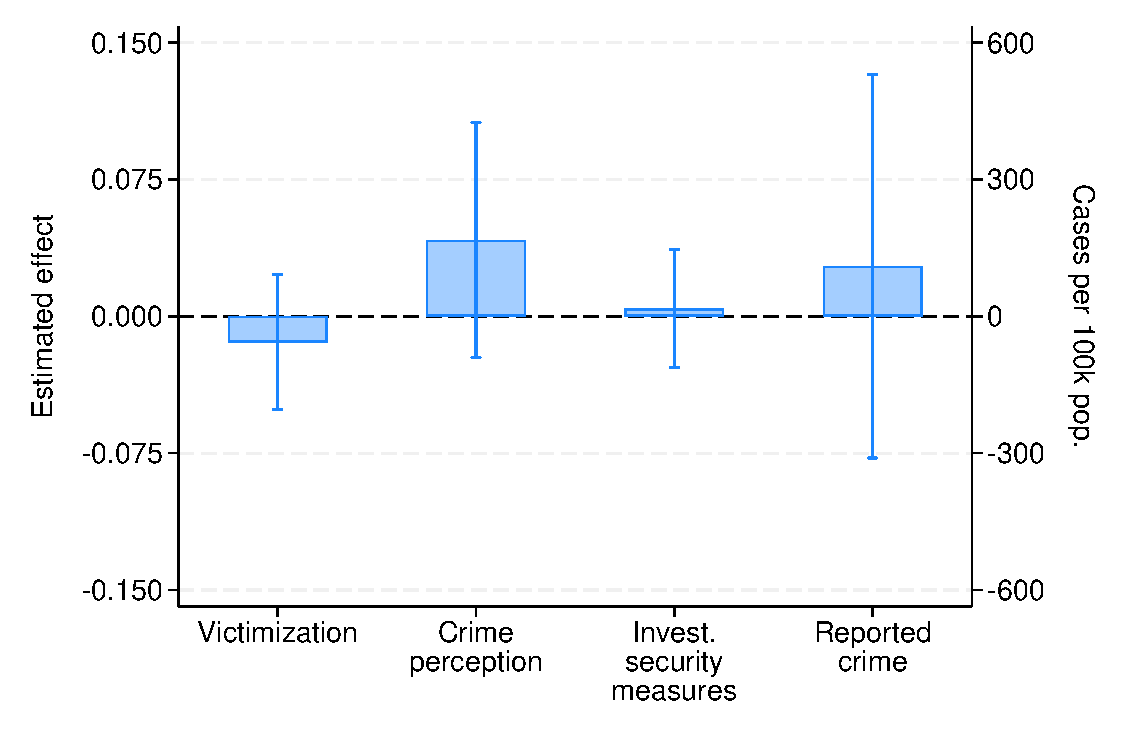
\includegraphics[width=\linewidth]{../manuscript/Graphs/results_SC_att_combined.pdf}
        \caption{Effects of \emph{Seguridad Ciudadana}}
    \end{subfigure}
    \\[6pt]
    \begin{subfigure}[t]{0.55\textwidth}
        \centering
        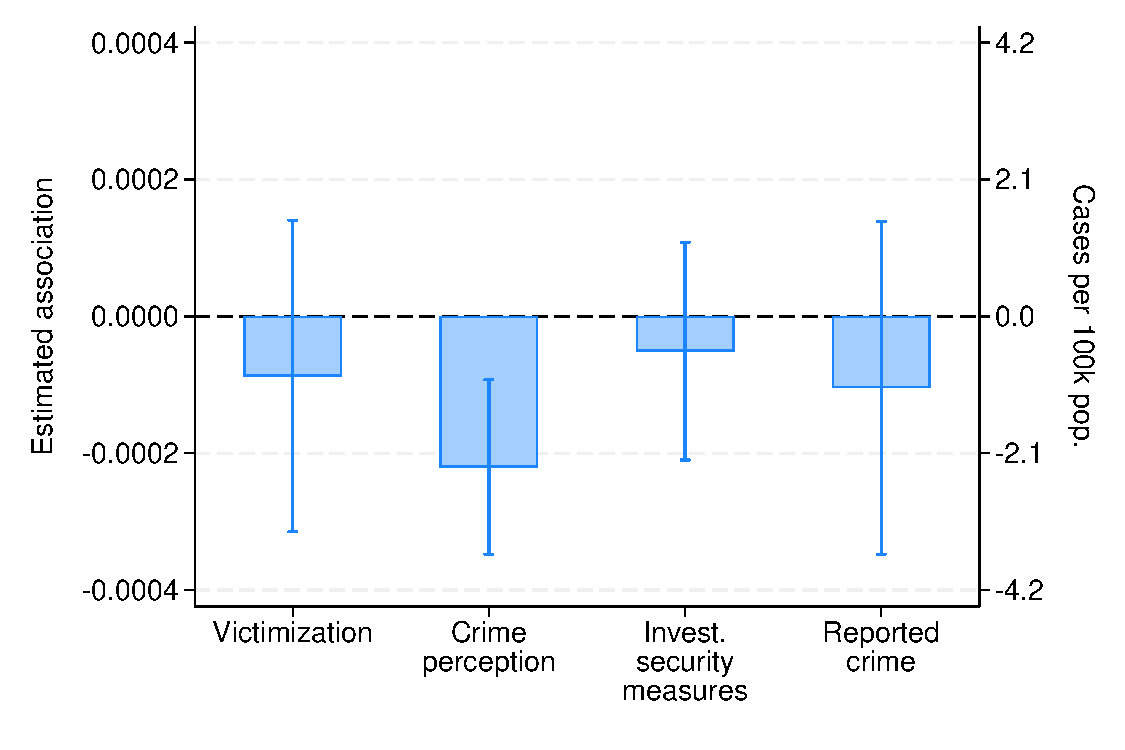
\includegraphics[width=\linewidth]{../manuscript/Graphs/results_corr_novariation_off_santiago.pdf}
        \caption{Association between police officers and effectiveness}
    \end{subfigure}
    \\[6pt]
    \begin{subfigure}[t]{0.55\textwidth}
        \centering
        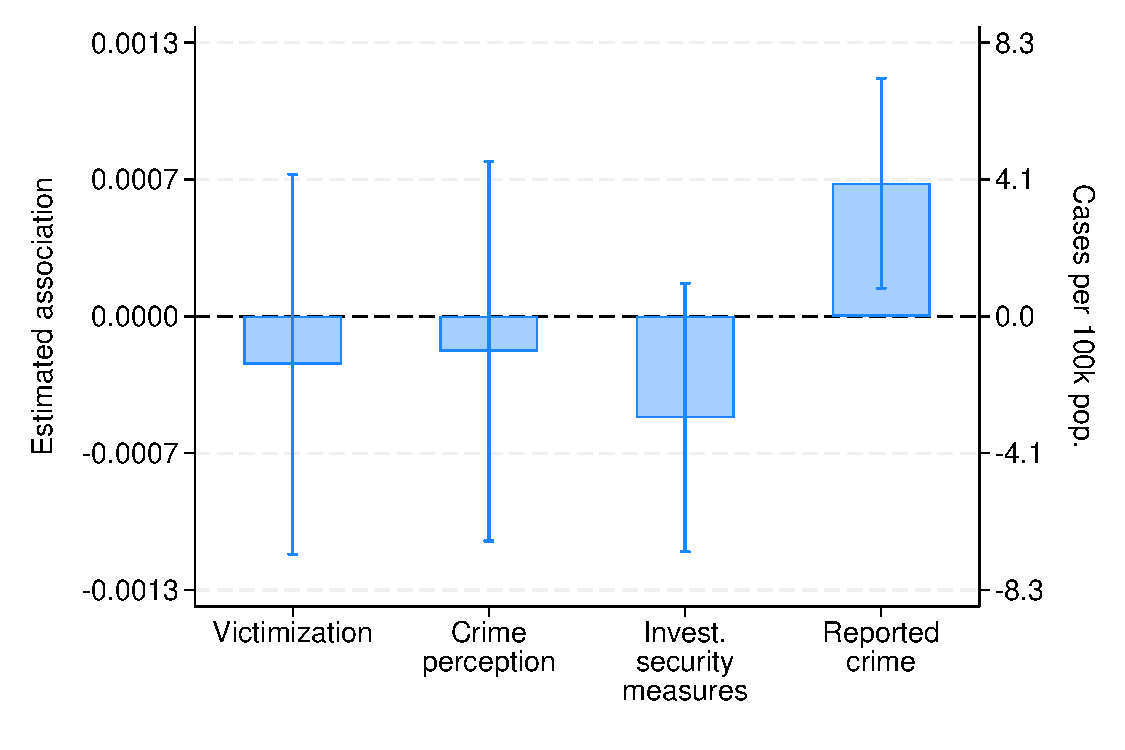
\includegraphics[width=\linewidth]{../manuscript/Graphs/results_corr_novariation_veh_santiago.pdf}
        \caption{Association between patrol vehicles and effectiveness}
    \end{subfigure}
    \\[8pt]
    \begin{minipage}{0.99\textwidth}
    \footnotesize Notes: Panel (a) reports the pooled effect of \emph{Seguridad Ciudadana}, a program that expanded local security personnel to support patrolling and deterrence but did not replicate the deployment-and-strategy features of \emph{Plan Cuadrante}. Panels (b) and (c) report within-municipality associations between police resources and police-effectiveness outcomes among the 41 municipalities of the Santiago Metropolitan Region, all of which had adopted \emph{Plan Cuadrante} by 2000. The regressions include municipality and year fixed effects. Standard errors are clustered at the municipality level using the wild bootstrapping procedure.
    \end{minipage}
\end{figure}